%===========
% bumpmapping

\section{Bump mapping}

Bump mapping je metoda pro zvýšení detailu povrchu.
V sekci normály \ref{subsec:normal} jsme si popsali interpolaci normály v bodě trojúhelníku.
Tímto přístupem získáme hladký povrch.
Zvýšení úrovně detailu bychom mohli dosáhnout zvětšením počtu polygonů.
Pokud bychom ale chtěli mít vyšší detaily uvnitř trojúhelníku, bez  přidání dalších trojúhelníků, můžeme zvolit bump mapping.
Bump mapping ovlivňuje normálu v bodě trojúhelníku a tím i výsledné stínování.
Pro ovlivňování normály se používá bump mapa.

Bump mapa je textura, která místo barvy nese informaci o normále.
Pokud bump mapu naneseme na trojúhelník a budeme pomocí ní ovlivňovat interpolovanou normálu, získáme vizuálně detailnější stínování.
Výsledek bump mappingu je znázorněn na obrázku \ref{fig:bump0}.
Bump mapa je tříkanálová textura.
Místo barev $(r,g,b)$ obsahuje složky normály $(u,v,w)$.
Bump mapu budeme vytvářet z textury těsně před obarvením.
Texturu v odstínech šedé budeme brát jako výškovou mapu a normála v daném bodě je na ní kolmá.
%TODO
\begin{figure}[h]
\centering
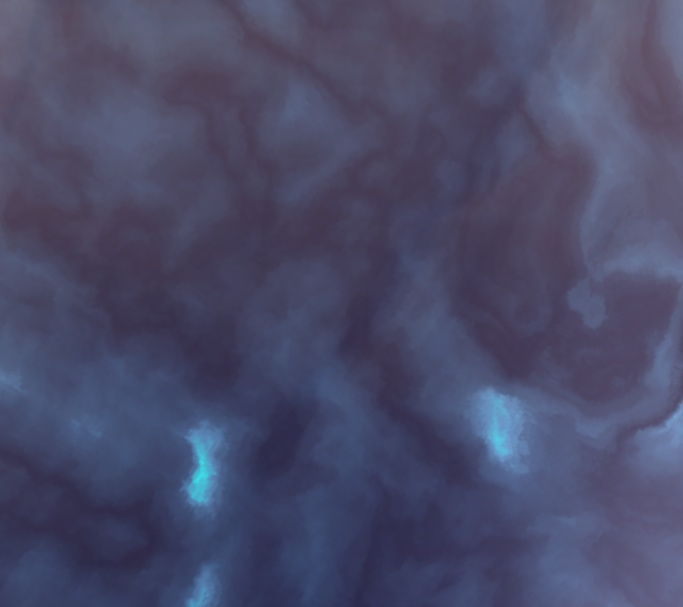
\includegraphics[width=4.9cm,keepaspectratio]{obr/bump0.jpg}
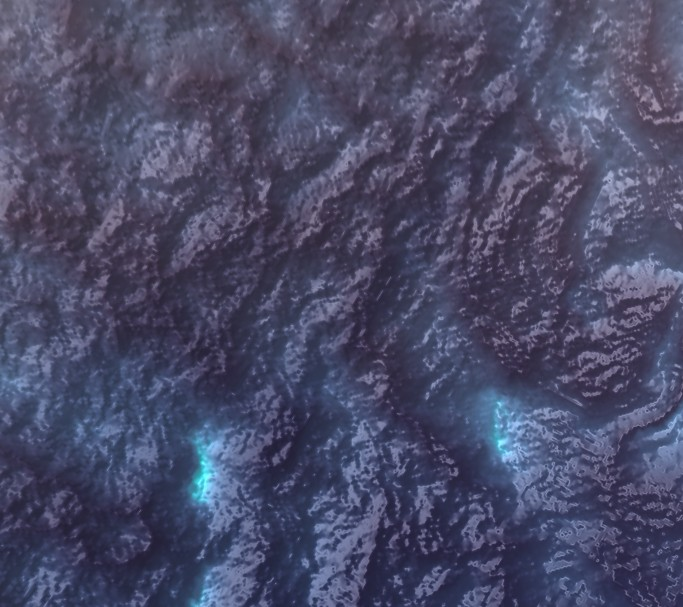
\includegraphics[width=4.9cm,keepaspectratio]{obr/bump1.jpg}
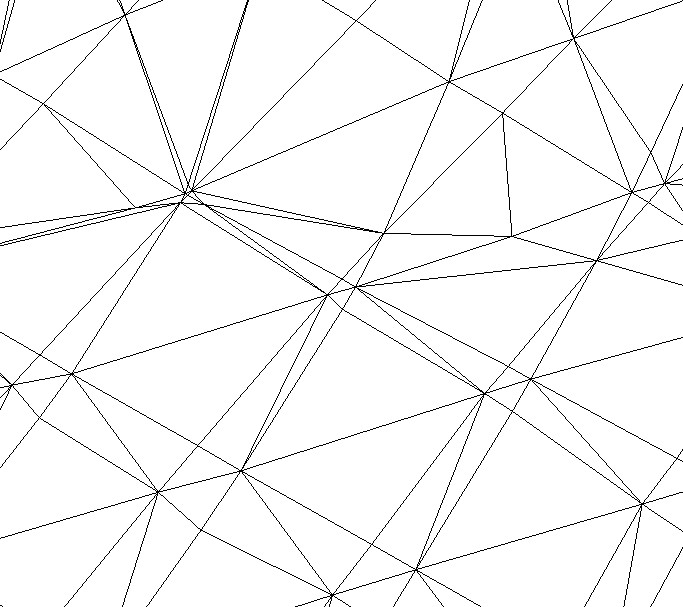
\includegraphics[width=4.9cm,keepaspectratio]{obr/bump2.jpg}
\caption{
Vlevo: Stínování s vyhlazením normál.
Uprostřed: stínování s aplikovaným bump mappingem.
Vpravo: trojúhelníková síť.}
\label{fig:bump0}
\end{figure}



